%%% Realiseirng for design af snubber-kredsløb til MOSFET og diode %%%

\subsection{Snubber-kredsløb}
For at teste realiseringen af snubber-kredsløbene måles MOSFET'ens drain spænding og diodens andode spænding. Først testes snubberen på primærsiden. Figur~\ref{fig:realiseirng_snubber_MOSFET_3} viser MOSFET'ens drain spænding. Her ses det, at den ønskede funktionalitet af den primære snubber er opnået. Signalet tager en enkelt svingning, og falder derefter til ro. Figur~\ref{fig:realiseirng_snubber_diode_3}, viser samme diodens anode spænding. Her ses det, at funktionalitet også er opnået ved det sekundære snubber-kredsløb. 

\begin{figure}[H]
	\center
	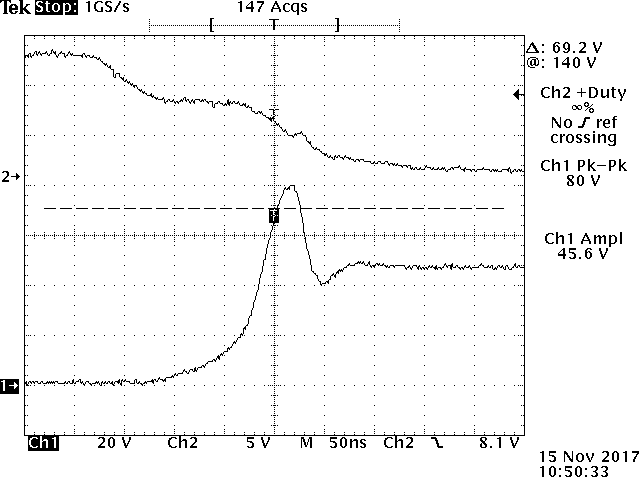
\includegraphics[max width=0.7\linewidth]{/tex/3iteration/billeder/Realisering/Realisering_snubber_MOSFET.PNG}
	\caption{Drain spænding efter snubber er tilføjet}
	\label{fig:realiseirng_snubber_MOSFET_3}
\end{figure} 

\begin{figure}[H]
	\center
	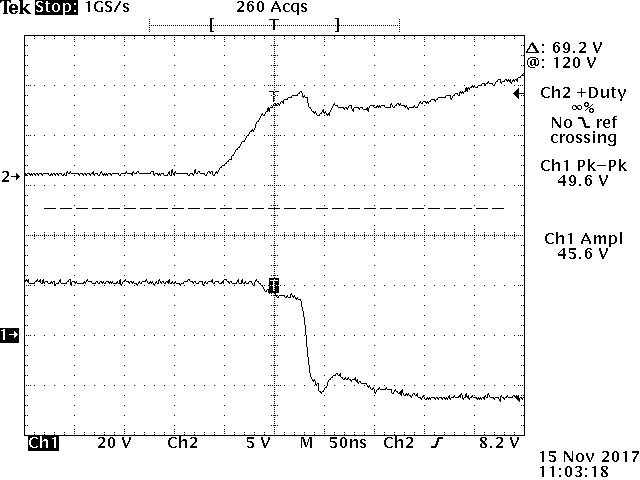
\includegraphics[max width=0.7\linewidth]{/tex/3iteration/billeder/Realisering/Realisering_snubber_diode.PNG}
	\caption{Anode spænding efter snubber er tilføjet}
	\label{fig:realiseirng_snubber_diode_3}
\end{figure} 

%TODO: Overvej nyt billede af dioden